\begin{frame}
\frametitle{Introduction}
\begin{columns}
    \column[t]{5cm}
	\begin{figure}[htbp!]
		\begin{center}
			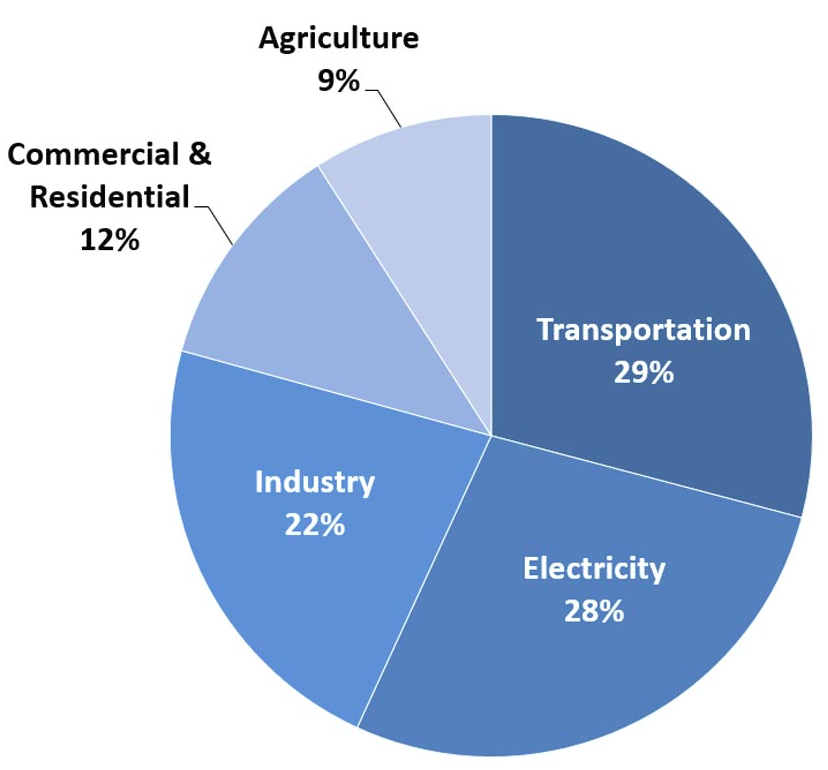
\includegraphics[height=5.0cm]{images/total-ghg-2017.png}
		\end{center}
		\caption{Total U.S. GHG Emissions by Economic Sector in 2017 \cite{us_epa_sources_2020}.}
	\end{figure}

	\column[t]{5cm}
	\\
	Illinois Climate Action Plan (iCAP):
	\begin{itemize}
		\item Main goal: carbon neutrality by 2050.
	\end{itemize}
	\vspace{0.75cm}
	Six target areas:
	\begin{itemize}
		\item Energy conservation.
		\item Energy generation, purchasing, and distribution.
		\item Transportation.
		\item Water and storm water.
		\item Waste and recycling.
		\item Agriculture, land use, and food.
	\end{itemize}
\end{columns}
\end{frame}

% Notes:
% Transportation and Electricity are the economic sectors that produced ...


\begin{frame}
\frametitle{Transportation}
\begin{columns}
	\column[t]{4.cm}
	\\
    Fuel Cell Electric Vehicles (FCEV):
	\begin{itemize}
		\item Address global warming concerns.
		\item Limitation on fossil fuel supply.
		\item Japan, Germany, and California.
		\item Champaign-Urbana.
	\end{itemize}

    \column[t]{6.cm}
	\begin{figure}[htbp!]
		\begin{center}
			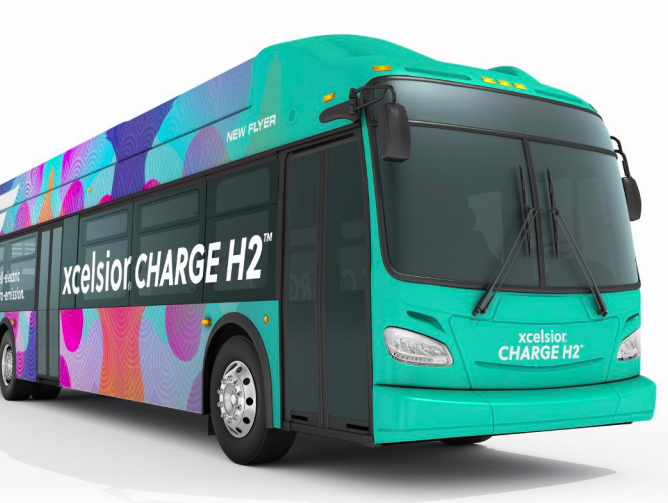
\includegraphics[height=5cm]{images/bus.png}
		\end{center}
		\caption{New Flyer fuel cell bus.}
	\end{figure}
\end{columns}
\end{frame}


\begin{frame}
\frametitle{Energy generation}
\begin{columns}
	\column[t]{4cm}
	\\
	Obvious solution:
	\begin{itemize}
		\item More renewables.
	\end{itemize}

    New problem:
	\begin{itemize}
		\item Duck curve.
		\item Demand ramps.
		\item Over-generation.
	\end{itemize}

    Consequences:
	\begin{itemize}
		\item Increase in dispatchable generation.
		\item Decrease in non-dispatchable generation.
	\end{itemize}

    \column[t]{6cm}
	\begin{figure}[htbp!]
		\begin{center}
			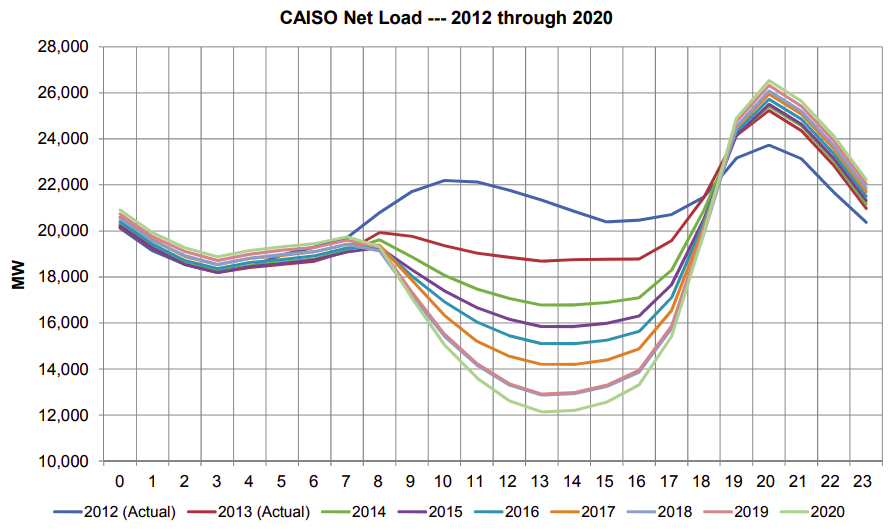
\includegraphics[height=4.0cm]{images/caiso-duck.png}
		\end{center}
		\caption{The duck curve.}
	\end{figure}
\end{columns}
\end{frame}


\begin{frame}
\frametitle{A possible solution}
\centering
    \textbf{Nuclear reactor and hydrogen:}
	\begin{itemize}
		\item Energy produced with no carbon emissions.
		\item Produce hydrogen as main/secondary product.
		\item Hydrogen as fuel for the FCEV.
		\item Hydrogen as electricity storage.
	\end{itemize}
	\vspace{1cm}
	\textbf{Approach consistent with our goal of reducing carbon emissions!!}
\end{frame}
